%definira klasu dokumenta 
\documentclass[12pt]{report} 

%prostor izmedu naredbi \documentclass i \begin{document} se zove uvod. U njemu se nalaze naredbe koje se odnose na cijeli dokument

%osnovni LaTex ne može riješiti sve probleme, pa se koriste različiti paketi koji olakšavaju izradu željenog dokumenta
\usepackage[croatian]{babel} 
\usepackage{amssymb}
\usepackage{amsmath}
\usepackage{txfonts}
\usepackage{mathdots}
\usepackage{titlesec}
\usepackage{array}
\usepackage{lastpage}
\usepackage{etoolbox}
\usepackage{longtable, tabu}
\usepackage{color, colortbl}
\usepackage{adjustbox}
\usepackage{geometry}
\usepackage[classicReIm]{kpfonts}
\usepackage{hyperref}
\usepackage{fancyhdr}

\usepackage{float}
\usepackage{setspace}
\restylefloat{table}


\patchcmd{\chapter}{\thispagestyle{plain}}{\thispagestyle{fancy}}{}{} %redefiniranje stila stranice u paketu fancyhdr

%oblik naslova poglavlja
\titleformat{\chapter}{\normalfont\huge\bfseries}{\thechapter.}{20pt}{\Huge}
\titlespacing{\chapter}{0pt}{0pt}{40pt}


\linespread{1.3} %razmak između redaka

\geometry{a4paper, left=1in, top=1in,}  %oblik stranice

\hypersetup{ colorlinks, citecolor=black, filecolor=black, linkcolor=black,	urlcolor=black }   %izgled poveznice


%prored smanjen između redaka u nabrajanjima i popisima
\newenvironment{packed_enum}{
	\begin{enumerate}
		\setlength{\itemsep}{0pt}
		\setlength{\parskip}{0pt}
		\setlength{\parsep}{0pt}
	}{\end{enumerate}}

\newenvironment{packed_item}{
	\begin{itemize}
		\setlength{\itemsep}{0pt}
		\setlength{\parskip}{0pt}
		\setlength{\parsep}{0pt}
	}{\end{itemize}}


%boja za privatni i udaljeni kljuc u tablicama
\definecolor{LightBlue}{rgb}{0.9,0.9,1}
\definecolor{LightGreen}{rgb}{0.9,1,0.9}


%podesavanje zaglavlja i podnožja

\pagestyle{fancy}
\lhead{Programsko inženjerstvo}
\rhead{Parkiraj Me}
\lfoot{seVen}
\cfoot{stranica \thepage/\pageref{LastPage}}
\rfoot{\today}
\renewcommand{\headrulewidth}{0.2pt}
\renewcommand{\footrulewidth}{0.2pt}


\begin{document} 
	
	
	
	\begin{titlepage}
		\begin{center}
			\vspace*{\stretch{1.0}} %u kombinaciji s ostalim \vspace naredbama definira razmak između redaka teksta
			\LARGE Programsko inženjerstvo\\
			\large Ak. god. 2020./2021.\\
			
			\vspace*{\stretch{3.0}}
			
			\huge Parkiraj Me\\
			\Large Dokumentacija, Rev. \textit{2}\\
			
			\vspace*{\stretch{12.0}}
			\normalsize
			Grupa: \textit{seVen}\\
			Voditelj: \textit{Marin Ćubela}\\
			
			
			\vspace*{\stretch{1.0}}
			Datum predaje: \textit{14. 1. 2021}\\
			
			\vspace*{\stretch{4.0}}
			
			Nastavnik: \textit{Nikolina Frid}\\
			
		\end{center}
		
		
	\end{titlepage}
	
	
	\tableofcontents
	
	\chapter{Dnevnik promjena dokumentacije}

\begin{longtabu} to \textwidth {|X[2, l]|X[13, l]|X[3, l]|X[3, l]|}
	\hline \multicolumn{1}{|l|}{\textbf{Rev.}}	& \multicolumn{1}{l|}{\textbf{Opis promjene/dodatka}} & \multicolumn{1}{|l|}{\textbf{Autori}} & \multicolumn{1}{l|}{\textbf{Datum}} \\[3pt] \hline
	\endfirsthead
	
	\hline \multicolumn{1}{|l|}{\textbf{Rev.}}	& \multicolumn{1}{l|}{\textbf{Opis promjene/dodatka}} & \multicolumn{1}{|l|}{\textbf{Autori}} & \multicolumn{1}{l|}{\textbf{Datum}} \\[3pt] \hline
	\endhead
	
	\hline 
	\endlastfoot
	
	0.1 & Preuzet predložak. & Ćubela & 20.10.2020. \\[3pt] \hline 
    0.2 & Dodan opis projektnog zadatka. & Matković, Strejček & 22.10.2020. \\[3pt] \hline 
    0.3 & Dodani obrasci uporabe. & Petković & 21.10.2020. \\[3pt] \hline
	0.4 & Dodani obrasci uporabe. & Bakić, Djaković & 25.10.2020. \\[3pt] \hline
	0.5 & Dodani dijagrami obrazaca uporabe. & Krišto, Ćubela & 29.10.2020. \\[3pt] \hline
	0.6 & Dodana dokumentacija za bazu podataka. & Krišto, Strejček & 5.11.2020. \\[3pt] \hline
	0.7 & Dodani sekvencijski dijagrami. & Djaković, Matković, Strejček & 10.11.2020. \\[3pt] \hline
	0.8 & Popravljeni obrasci uporabe & Bakić, Matković, Strejček & 12.11.2020. \\[3pt] \hline
	0.9 & Popravljeni dijagrami & Krišto, Strejček & 13.11.2020. \\[3pt] \hline
	1.0 & Dodane upute za puštanje u pogon i korištene tehnologije i alati& Djaković & 12.01.2021. \\[3pt] \hline
	1.1 & Dodani dijagrami(act, stm, cmp) i popravljeni obrasci uporabe& Matković, Strejček & 13.01.2021. \\[3pt] \hline

	&  &  & \\[3pt] \hline

	
\end{longtabu}
	\chapter{Opis projektnog zadatka}

Cilj projekta je razviti programsku podršku za stvaranje web aplikacije \textit {Parkiraj me}. Aplikacija će korisniku omogućiti praćenje stanja slobodnih parkirališnih mjesta na svim lokacijama diljem Zagreba u stvarnom vremenu te jednokratnu, ponavljajuću ili trajnu rezervaciju parkirališnog mjesta. Putem aplikacije sve zainteresirane tvrtke moći će ponuditi svoja parkirališta na kojima će korisnici kasnije moći rezervirati svoja mjesta.

Pokretanjem aplikacije prikazuje se karta s prikazanim dostupnim parkiralištima i brojem slobodnih parkirališnih mjesta te opcija za registraciju ili prijavu u sustav.\newline 
Neprijavljeni korisnik može se prijaviti na postojeći račun (mora upisati e-mail adresu i lozinku). Neregistrirani korisnik ima mogućnost registracije kao: \textit{Klijent} (rezervira parkirališna mjesta) ili \textit{Tvrtka} (ovlašteni zaposlenik tvrtke).
\newline
Za klijenta potrebni podaci za registraciju su:
\begin{itemize}
    \item OIB
    \item Ime i prezime
    \item E-mail adresa
    \item Lozinka
    \item Broj kreditne kartice
\end{itemize}
Za tvrtku potrebni podaci za registraciju su:
\begin{itemize}
    \item OIB
    \item Naziv tvrtke
    \item E-mail adresa
    \item Lozinka
    \item Adresa sjedišta
\end{itemize}

\textit{\underbar{Klijent}} je registrirani korisnik stariji od 18 godina, koji ima pravo rezervirati parkirno mjesto. Klijent na karti odabire parkiralište na kojem želi rezervirati mjesto i dobiva informaciju o broju slobodnih mjesta. Druga mogućnost je da na temelju trenutne lokacije aplikacija daje prijedlog najbližih parkirališta sa slobodnim parkirnim mjestima (prednost imaju parkirališta s brojem slobodnih mjesta većim od 10). Ukoliko odabrano parkiralište ima slobodnih mjesta odabire mogućnost rezervacije. Nakon toga klijent bira tip rezervacije koju želi i odabire vozilo za koje želi izvršiti rezervaciju. Rezervacija se naplaćuje izravnim terećenjem njegove kreditne kartice. Potvrdom plaćanja aktivira se rezervacija u sustavu. 

Klijent istovremeno može imati više različitih tipova rezervacija, na različitim parkiralištima s različitim vozilima.

\textit{\underbar{Tvrtka}} je korisnik kojeg prijavljuje ovlašteni zaposlenik tvrtke. Ovlašteni zaposlenik nakon registracije svoje tvrtke unosi podatke o parkiralištima koje nudi ta tvrtka. Odabirom opcije za dodavanje parkirališta unosi se:
\begin{itemize}
    \item ime parkirališta
    \item lokacija parkirališta
    \item tip parkirališta (otvoreno ili zatvoreno)
    \item ukupni broj mjesta 
    \item broj invalidskih mjesta (potrebno za određivanje broja slobodnih mjesta)
    \item cijena parkinga
\end{itemize}
 Preduvjet za prijavu parkirališta je opremljenost pametnim kamerama na svakom parkirališnom mjestu kako bi se prepoznala zauzeta mjesta te kako bi se mogla očitati registracija vozila na parkirališnom mjestu. Nakon uspješne prijave parkirališta, to parkiralište postaje vidljivo svim korisnicima aplikacije na karti te su na njemu moguće rezervacije.
\newline

\textit{\underbar{Administrator}} sustava upravlja svim korisnicima aplikacije. On ima pristup popisu svih registriranih korisnika i njihovih osnovnih podataka (ime, prezime, e-mail adresa, popis vozila). Ima pristup popisu rezervacija,
također može potvrditi dodavanje ili brisanje parkirališta.
\newpage\textit{Upravljanje korisničkim računom}

Korisnici imaju mogućnost upravljanja svojim računima, pregledavanjem, uređivanjem i brisanjem svojeg računa.

Klijent ima pregled svih svojih prijavljenih vozila. Svako vozilo ima svoju registraciju, ime i boju. Vozilo klijent može uređivati (promjenom registracije, imena ili boje vozila). Može dodavati nova vozila ili postojeća obrisati. 

Klijent ima prijavljenu kreditnu karticu. Karticu može uređivati u slučaju pogrešnog unosa i postojeću zamijeniti novom, dakle izbrisati staru i stvoriti novu. Klijent uvijek treba imati prijavljenu jednu karticu.

Tvrtka ima pregled vlastitih parkirališta. Svako parkiralište može uređivati, može dodavati nova parkirališta ili brisati postojeća. 
\newline
\newline
\textit{Rezervacija}

Parkirno mjesto se može rezervirati jednokratno, kao ponavljajuća rezervacija ili kao trajna rezervacija. Svaka rezervacija ima svoj jedinstveni id. Cijena rezervacije ovisi o tipu rezervacije i cjeniku pojedinog parkirališta.

\textit{\underbar{Jednokratna rezervacija}} se rezervira za vremenski period kraći od 24 sata i rezervacija se mora obaviti barem 6 sati unaprijed. Plaćanje se vrši odmah u trenutku rezervacije.

\textit{\underbar{Ponavljajuća rezervacija}} mora trajati najmanje 1 sat i mora se ponavljati barem jednom tjedno tijekom mjesec dana. Plaćanje se vrši svakih 30 dana.

\textit{\underbar{Trajna rezervacija}} odnosi se na rezervaciju parkirališnog mjesta 0-24 sata svaki dan na neodređeni period. Plaćanje se vrši svakih 30 dana.
\newline
\newline
\textit{Dodatno:}

Ukoliko se briše korisnički račun neke tvrtke, brišu se sva njena parkirališta, a za sve korisnike ukida se rezervacija ako postoji na tim parkiralištima. Ukoliko ima preostalog neiskorištenog rezerviranog vremena korisniku se vraća novac.

Sustav treba podržavati rad više korisnika u stvarnom vremenu.

	\chapter{Specifikacija programske potpore}

\section{Funkcionalni zahtjevi}			

\noindent \textbf{Dionici:}

\begin{packed_enum}
	
	\item Ovlašteni zaposlenik tvrtke
	\item Klijent
	\item Administrator
	\item Razvojni tim
	
\end{packed_enum}

\noindent \textbf{Aktori i njihovi funkcionalni zahtjevi:}


\begin{packed_enum}
	\item  \underbar{Neregistrirani/neprijavljeni korisnik (inicijator) može:}
	
	\begin{packed_enum}
		
		\item vidjeti kartu s parkiralištima (adresa, broj ukupnih i slobodnih mjesta, cijena)
		\item registrirati se i/ili prijaviti se (kao klijent ili tvrtka)
		
	\end{packed_enum}
	
	\item  \underbar{Klijent (inicijator) može:}
	
	\begin{packed_enum}
		
		\item vidjeti kartu s parkiralištima (adresa, broj ukupnih i slobodnih mjesta, cijena)
		\item pregledavati, uređivati i izbrisati korisnički račun
		\item pregledavati, uređivati i izbrisati vozila
		\item pregledavati, uređivati i izbrisati kartice
		\item rezervirati parkirališno mjesto
		\item pregledavati, uređivati i izbrisati rezervacije
		\item pisati i pregledavati  recenzije
		\item tražiti upute do parkirališta
		
	\end{packed_enum}
	
	
	\item  \underbar{Ovlašteni zaposlenik tvrtke (inicijator) može:}
	
	\begin{packed_enum}
		
		\item vidjeti kartu s parkiralištima
		\item pregledavati, uređivati, dodavati i brisati svoja parkirališta
		\item pregledavati, uređivati i izbrisati korisnički račun
		\item pregledavati vlastite i tuđe recenzije
		\item pregledavati rezervacije na vlastitim parkiralištima
		\item odgovoriti na recenzije korisnika
		
	\end{packed_enum}
	
	\item \underbar{Administrator (inicijator) može:}
	
	\begin{packed_enum}
		
		\item vidjeti popis svih registriranih korisnika i osnovnih podataka
		\item pregledavati rezervacije
		\item brisati i mijenjati razinu pristupa aplikaciji drugim korisnicima
		\item brisati recenzije
		\item dodavati ili brisati parkirališta
		
	\end{packed_enum}
	
	\item \underbar{Baza podataka (sudionik) može:}
	
	\begin{packed_enum}
		
		\item pohranjivati podatke o korisnicima (osobni podatci, kartica, vozila)
		\item pohranjivati podatke o parkiralištima (njihovim kapacitetima i ponudama)
		\item pohranjivati podatke o rezervacijama
		\item pohranjivati podatke o tvrtkama
		
	\end{packed_enum}
\end{packed_enum}


\eject 



\subsection{Obrasci uporabe}

\subsubsection{Opis obrazaca uporabe}

\noindent \underbar{\textbf{UC1 - Pristup privatnim rutama}}
\begin{packed_item}
	
	\item \textbf{Glavni sudionik:} Korisnik
	\item \textbf{Cilj:} Zabraniti pristup privatnim rutama
	\item \textbf{Sudionici:} -
	\item \textbf{Preduvjet:} Korisnik nije prijavljen
	\item \textbf{Opis osnovnog tijeka:}
	
	\item[] \begin{packed_enum}
		
		\item Pristup privatnoj ruti se zabranjuje te se korisnik preusmjerava na formu za prijavu
		\item Korisnik se prijavljuje te se preusmjerava na prethodnu zabranjenu rutu
	\end{packed_enum}
	
	\item  \textbf{Opis mogućih odstupanja:}
	
	\item[] \begin{packed_item}
		
		\item[2.a] Korisnik pokušava pristupiti rutama koje njemu nisu dostupne
		\item[] \begin{packed_enum}
			
			\item Nakon prijave korisnik se preusmjerava na početni zaslon aplikacije
			
		\end{packed_enum}
		
	\end{packed_item}
\end{packed_item}

\noindent \underbar{\textbf{UC$<$broj obrasca$>$ -$<$ime obrasca$>$}}
\begin{packed_item}
	
	\item \textbf{Glavni sudionik: }$<$sudionik$>$
	\item  \textbf{Cilj:} $<$cilj$>$
	\item  \textbf{Sudionici:} $<$sudionici$>$
	\item  \textbf{Preduvjet:} $<$preduvjet$>$
	\item  \textbf{Opis osnovnog tijeka:}
	
	\item[] \begin{packed_enum}
		
		\item $<$opis korak jedan$>$
		\item $<$opis korak dva$>$
		\item $<$opis korak tri$>$
		\item $<$opis korak četiri$>$
		\item $<$opis korak pet$>$
	\end{packed_enum}
	
	\item  \textbf{Opis mogućih odstupanja:}
	
	\item[] \begin{packed_item}
		
		\item[2.a] $<$opis mogućeg scenarija odstupanja u koraku 2$>$
		\item[] \begin{packed_enum}
			
			\item $<$opis rješenja mogućeg scenarija korak 1$>$
			\item $<$opis rješenja mogućeg scenarija korak 2$>$
			
		\end{packed_enum}
		\item[2.b] $<$opis mogućeg scenarija odstupanja u koraku 2$>$
		\item[3.a] $<$opis mogućeg scenarija odstupanja  u koraku 3$>$
		
	\end{packed_item}
\end{packed_item}

\subsubsection{Dijagrami obrazaca uporabe}

\textit{Prikazati odnos aktora i obrazaca uporabe odgovarajućim UML dijagramom. Nije nužno nacrtati sve na jednom dijagramu. Modelirati po razinama apstrakcije i skupovima srodnih funkcionalnosti.}
\eject		

\subsection{Sekvencijski dijagrami}

\textbf{\textit{dio 1. revizije}}\\

\textit{Nacrtati sekvencijske dijagrame koji modeliraju najvažnije dijelove sustava (max. 4 dijagrama). Ukoliko postoji nedoumica oko odabira, razjasniti s asistentom. Uz svaki dijagram napisati detaljni opis dijagrama.}
\eject

\section{Ostali zahtjevi}

\textbf{\textit{dio 1. revizije}}\\

\textit{Nefunkcionalni zahtjevi i zahtjevi domene primjene dopunjuju funkcionalne zahtjeve. Oni opisuju \textbf{kako se sustav treba ponašati} i koja \textbf{ograničenja} treba poštivati (performanse, korisničko iskustvo, pouzdanost, standardi kvalitete, sigurnost...). Primjeri takvih zahtjeva u Vašem projektu mogu biti: podržani jezici korisničkog sučelja, vrijeme odziva, najveći mogući podržani broj korisnika, podržane web/mobilne platforme, razina zaštite (protokoli komunikacije, kriptiranje...)... Svaki takav zahtjev potrebno je navesti u jednoj ili dvije rečenice.}




	\chapter{Arhitektura i dizajn sustava}
		
		\textbf{\textit{dio 1. revizije}}\\

		\textit{ Potrebno je opisati stil arhitekture te identificirati: podsustave, preslikavanje na radnu platformu, spremišta podataka, mrežne protokole, globalni upravljački tok i sklopovsko-programske zahtjeve. Po točkama razraditi i popratiti odgovarajućim skicama:}
	\begin{itemize}
		\item 	\textit{izbor arhitekture temeljem principa oblikovanja pokazanih na predavanjima (objasniti zašto ste baš odabrali takvu arhitekturu)}
		\item 	\textit{organizaciju sustava s najviše razine apstrakcije (npr. klijent-poslužitelj, baza podataka, datotečni sustav, grafičko sučelje)}
		\item 	\textit{organizaciju aplikacije (npr. slojevi frontend i backend, MVC arhitektura) }		
	\end{itemize}

	
		

		

		\pagebreak		
		\section{Baza podataka}
			
		Za naš sustav koristit ćemo relacijsku bazu podataka koja svojom strukturom olakšava modeliranje stvarnog svijeta. Gradivna jedinka baze je relacija, odnosno tablica koja je definirana svojim imenom i skupom atributa. Zadaća baze podataka je brza i jednostavna pohrana, izmjena i dohvat podataka za daljnju obradu.
		\newline
        Baza podataka ove aplikacije sastoji se od sljedećih entiteta: 
        \begin{itemize}
            \item Račun
            \item Klijent
            \item Tvrtka
            \item Vozilo
            \item Parkiralište
            \item Rezervacija
            \item Jednokratna
            \item Trajna
            \item Ponavljajuća
        \end{itemize}
        
		
			\subsection{Opis tablica}
			
			    \textbf{Račun} \newline
			    Entitet sadrži informacije o napravljenom računu u aplikaciji. Sadrži
			    atribute: ID, email, OIB, admin, lozinka. U vezi je \textit{One-To-Many} s entitetima Klijent i Tvrtka.
				
				\begin{longtabu} to \textwidth {|X[6, l]|X[6, l]|X[20, l]|}
					
					\hline \multicolumn{3}{|c|}{\textbf{Račun}}	 \\[3pt] \hline
					\endfirsthead
					
					\hline \multicolumn{3}{|c|}{\textbf{Račun}}	 \\[3pt] \hline
					\endhead
					
					\hline 
					\endlastfoot
					
					\cellcolor{LightGreen}ID & INT	&  jedinstveni identifikator računa \\ \hline
					email & VARCHAR &  e-mail adresa računa \\ \hline 
					OIB	& CHAR(11) &   oib osobe čiji je račun	\\ \hline 
					admin & BOOLEAN	&  	true ako je osoba administrator	\\ \hline 
					lozinka & VARCHAR	&  	hash lozinke	\\ \hline 
					
					
				\end{longtabu}
				
				\pagebreak
				\textbf{Klijent} \newline
			    Entitet sadrži informacije o klijentu koji koristi aplikaciju. Sadrži
			    atribute: ID, ime, prezime, broj kartice, računId. U vezi je \textit{One-To-Many} s entitetima Vozilo i Rezervacija, a s entitetom Račun je u vezi \textit{Many-To-One}.
				
				\begin{longtabu} to \textwidth {|X[6, l]|X[6, l]|X[20, l]|}
					
					\hline \multicolumn{3}{|c|}{\textbf{Klijent}}	 \\[3pt] \hline
					\endfirsthead
					
					\hline \multicolumn{3}{|c|}{\textbf{Klijent}}	 \\[3pt] \hline
					\endhead
					
					\hline 
					\endlastfoot
					
					\cellcolor{LightGreen}ID & INT	&  jedinstveni identifikator klijenta \\ \hline
					ime & VARCHAR &  ime klijenta \\ \hline 
					prezime & VARCHAR &  prezime klijenta \\ \hline 
					broj kartice & VARCHAR &  broj kartice klijenta \\ \hline 
					\cellcolor{LightBlue} računId	& VARCHAR &   jedinstveni identifikator računa (račun.ID)	\\ \hline 
					
					
				\end{longtabu}
				
				\textbf{Tvrtka} \newline
			    Entitet sadrži informacije o tvrtki koja želi prijaviti svoje parkilište u aplikaciji. Sadrži atribute: ID, naziv, adresa, računId. U vezi je \textit{One-To-Many} s entitetom Parkiralište, a s entitetom Račun je u vezi \textit{Many-To-One}.
				
				\begin{longtabu} to \textwidth {|X[6, l]|X[6, l]|X[20, l]|}
					
					\hline \multicolumn{3}{|c|}{\textbf{Tvrtka}}	 \\[3pt] \hline
					\endfirsthead
					
					\hline \multicolumn{3}{|c|}{\textbf{Tvrtka}}	 \\[3pt] \hline
					\endhead
					
					\hline 
					\endlastfoot
					
					\cellcolor{LightGreen}ID & INT	&  jedinstveni identifikator tvrtke \\ \hline
					naziv & VARCHAR &  naziv tvrtke \\ \hline 
					adresa & VARCHAR &  adresa sjedišta tvrtke \\ \hline 
					\cellcolor{LightBlue} računId	& VARCHAR &   jedinstveni identifikator računa (račun.ID)	\\ \hline 
					
					
				\end{longtabu}
				
				\textbf{Vozilo} \newline
			    Entitet sadrži informacije o vozilo kojeg je klijent prijavio. Sadrži
			    atribute: ID, registracija, naziv vozila, boja, i klijentId. U vezi je \textit{One-To-Many} s entitetom Rezervacija, a s entitetom Klijent je u vezi \textit{Many-To-One}.
				
				\begin{longtabu} to \textwidth {|X[6, l]|X[6, l]|X[20, l]|}
					
					\hline \multicolumn{3}{|c|}{\textbf{Vozilo}}	 \\[3pt] \hline
					\endfirsthead
					
					\hline \multicolumn{3}{|c|}{\textbf{Vozilo}}	 \\[3pt] \hline
					\endhead
					
					\hline 
					\endlastfoot
					
					\cellcolor{LightGreen}ID & INT	&  jedinstveni identifikator vozila \\ \hline
					registracija & VARCHAR &  broj registracije vozila \\ \hline 
					naziv vozila & VARCHAR &  naziv vozila koje dodjeluje klijent \\ \hline 
					boja & VARCHAR &  boja vozila koju dodjeluje klijent \\ \hline 
					\cellcolor{LightBlue} klijentId	& VARCHAR &   jedinstveni identifikator klijenta (klijent.ID)	\\ \hline 
					
				\end{longtabu}
				
				\pagebreak
				\textbf{Parkiralište} \newline
			    Entitet sadrži informacije o parkiralištu neke tvrtke koje se nudi klijentima. Sadrži
			    atribute: ID, naziv, broj mjesta, broj invalidskih mjesta, tip prakirališta, koordinate, cijena jednokratne, cijena ponavljajuće, cijena trajne i tvrtkaId. U vezi je \textit{One-To-Many} s entitetom Rezervacija, a s entitetom Tvrtka je u vezi \textit{Many-To-One}.
				
				\begin{longtabu} to \textwidth {|X[6, l]|X[6, l]|X[20, l]|}
					
					\hline \multicolumn{3}{|c|}{\textbf{Parkiralište}}	 \\[3pt] \hline
					\endfirsthead
					
					\hline \multicolumn{3}{|c|}{\textbf{Parkiralište}}	 \\[3pt] \hline
					\endhead
					
					\hline 
					\endlastfoot
					
					\cellcolor{LightGreen}ID & INT	&  jedinstveni identifikator parkirališta \\ \hline
					naziv & VARCHAR &  naziv parkirališta \\ \hline 
					broj mjesta & INT &  broj mjesta koje parkiralište nudi \\ \hline 
					broj invalidskih mjesta & INT &  broj invalidskih mjesta koje ima parkiralište \\ \hline tip parkirališta & VARCHAR &  tip parkirališta (otvoreno, zatvoreno) \\ \hline 
					koordinate & VARCHAR &  zemljopisna dužina i širina parkirališta \\ \hline 
					cijena jednokratne & INT &  cijena sata za jednokratnu rezervaciju parkirališta \\ \hline 
					cijena ponavljajuće & INT &  cijena sata za ponavljajuću rezervaciju parkirališta \\ \hline
					cijena trajne & INT &  cijena trajne rezervacije parkirališta \\ \hline
					\cellcolor{LightBlue} tvrtkaId	& VARCHAR &   jedinstveni identifikator tvrtke (tvrka.ID)	\\ \hline 
					
					
				\end{longtabu}
				
				
				\textbf{Rezervacija} \newline
			    Entitet sadrži informacije o stvorenoj rezervaciji u aplikaciji. Ima
			    atribute: ID, klijentId, parkirališteId, voziloId. U vezi je \textit{One-To-Many} s entitetima Jednokratna, Ponavljajuća i Trajna. S entitetima Klijent, Parkiralište i Vozilo je u vezi \textit{Many-To-One}.
				
				\begin{longtabu} to \textwidth {|X[6, l]|X[6, l]|X[20, l]|}
					
					\hline \multicolumn{3}{|c|}{\textbf{Rezervacija}}	 \\[3pt] \hline
					\endfirsthead
					
					\hline \multicolumn{3}{|c|}{\textbf{Rezervacija}}	 \\[3pt] \hline
					\endhead
					
					\hline 
					\endlastfoot
					
					\cellcolor{LightGreen}ID & INT	&  jedinstveni identifikator rezervacije \\ \hline
					\cellcolor{LightBlue} klijentId	& VARCHAR &   jedinstveni identifikator klijenta (klijent.ID)	\\ \hline
					\cellcolor{LightBlue} parkirališteId	& VARCHAR &   jedinstveni identifikator prakirališta (parkiralište.ID)	\\ \hline
					\cellcolor{LightBlue} voziloId	& VARCHAR &   jedinstveni identifikator vozila (vozilo.ID)	\\ \hline
					
				\end{longtabu}
				
				\pagebreak
				\textbf{Jednokratna} \newline
			    Entitet sadrži informacije o jednokratnoj rezervaciji stvorenoj u aplikaciji. Ima
			    atribute: ID, vrijeme početak, vrijeme kraj, rezervaijaId. U vezi je \textit{Many-To-One} s entitetom Rezervacija.
			    
				\begin{longtabu} to \textwidth {|X[6, l]|X[6, l]|X[20, l]|}
					
					\hline \multicolumn{3}{|c|}{\textbf{Jednokratna}}	 \\[3pt] \hline
					\endfirsthead
					
					\hline \multicolumn{3}{|c|}{\textbf{Jednokratna}}	 \\[3pt] \hline
					\endhead
					
					\hline 
					\endlastfoot
					
					\cellcolor{LightGreen}ID & INT	&  jedinstveni identifikator jednokratne rezervacije \\ \hline
					vrijeme početak & TIMESTAMP &  vrijeme početka rezervacije \\ \hline  
					vrijeme kraj & TIMESTAMP &  vrijeme kraja rezervacije \\ \hline 
					\cellcolor{LightBlue} rezervacijaId	& VARCHAR &   jedinstveni identifikator rezervacije (rezervacija.ID)	\\ \hline
					
				\end{longtabu}
				
				\textbf{Trajna} \newline
			    Entitet sadrži informacije o trajnoj rezervaciji stvorenoj u aplikaciji. Ima
			    atribute: ID, vrijeme početak, vrijeme kraj, rezervaijaId. U vezi je \textit{Many-To-One} s entitetom Rezervacija.
				
				\begin{longtabu} to \textwidth {|X[6, l]|X[6, l]|X[20, l]|}
					
					\hline \multicolumn{3}{|c|}{\textbf{Trajna}}	 \\[3pt] \hline
					\endfirsthead
					
					\hline \multicolumn{3}{|c|}{\textbf{Trajna}}	 \\[3pt] \hline
					\endhead
					
					\hline 
					\endlastfoot
					
					\cellcolor{LightGreen}ID & INT	&  jedinstveni identifikator trajne rezervacije \\ \hline
					vrijeme početak & TIMESTAMP &  vrijeme početka rezervacije \\ \hline  
					vrijeme kraj & TIMESTAMP &  vrijeme kraja rezervacije \\ \hline 
					\cellcolor{LightBlue} rezervacijaId	& VARCHAR &   jedinstveni identifikator rezervacije (rezervacija.ID)	\\ \hline
					
				\end{longtabu}
				
				\pagebreak
				\textbf{Ponavljajuća} \newline
			    Entitet sadrži informacije o ponavljaućoj rezervaciji stvorenoj u aplikaciji. Ima
			    atribute: ID, datum rezervacije, datum kraja rezervcije, dani ponavljanja, vrijeme početak, vrijeme kraj i rezervaijaId. U vezi je \textit{Many-To-One} s entitetom Rezervacija.
				
				\begin{longtabu} to \textwidth {|X[6, l]|X[6, l]|X[20, l]|}
					
					\hline \multicolumn{3}{|c|}{\textbf{Ponavljajuća}}	 \\[3pt] \hline
					\endfirsthead
					
					\hline \multicolumn{3}{|c|}{\textbf{Ponavljajuća}}	 \\[3pt] \hline
					\endhead
					
					\hline 
					\endlastfoot
					
					\cellcolor{LightGreen}ID & INT	&  jedinstveni identifikator ponavljajuće rezervacije \\ \hline
					datum rezervacije & DATE &  datum početka rezervacije \\ \hline
					datum kraja rezervacije & DATE &  datum kraja rezervacije \\ \hline
					dani ponavljanja & INT &  dani ponavljanje rezervacije (pon=1, uto=2, ...) \\ \hline
					vrijeme početak & TIME &  vrijeme početka rezervacije \\ \hline  
					vrijeme kraj & TIME &  vrijeme kraja rezervacije \\ \hline 
					\cellcolor{LightBlue} rezervacijaId	& VARCHAR &   jedinstveni identifikator rezervacije (rezervacija.ID)	\\ \hline
					
				\end{longtabu}
				
				
			
			\pagebreak
			\subsection{Dijagram baze podataka}
                \begin{figure}[H]
                	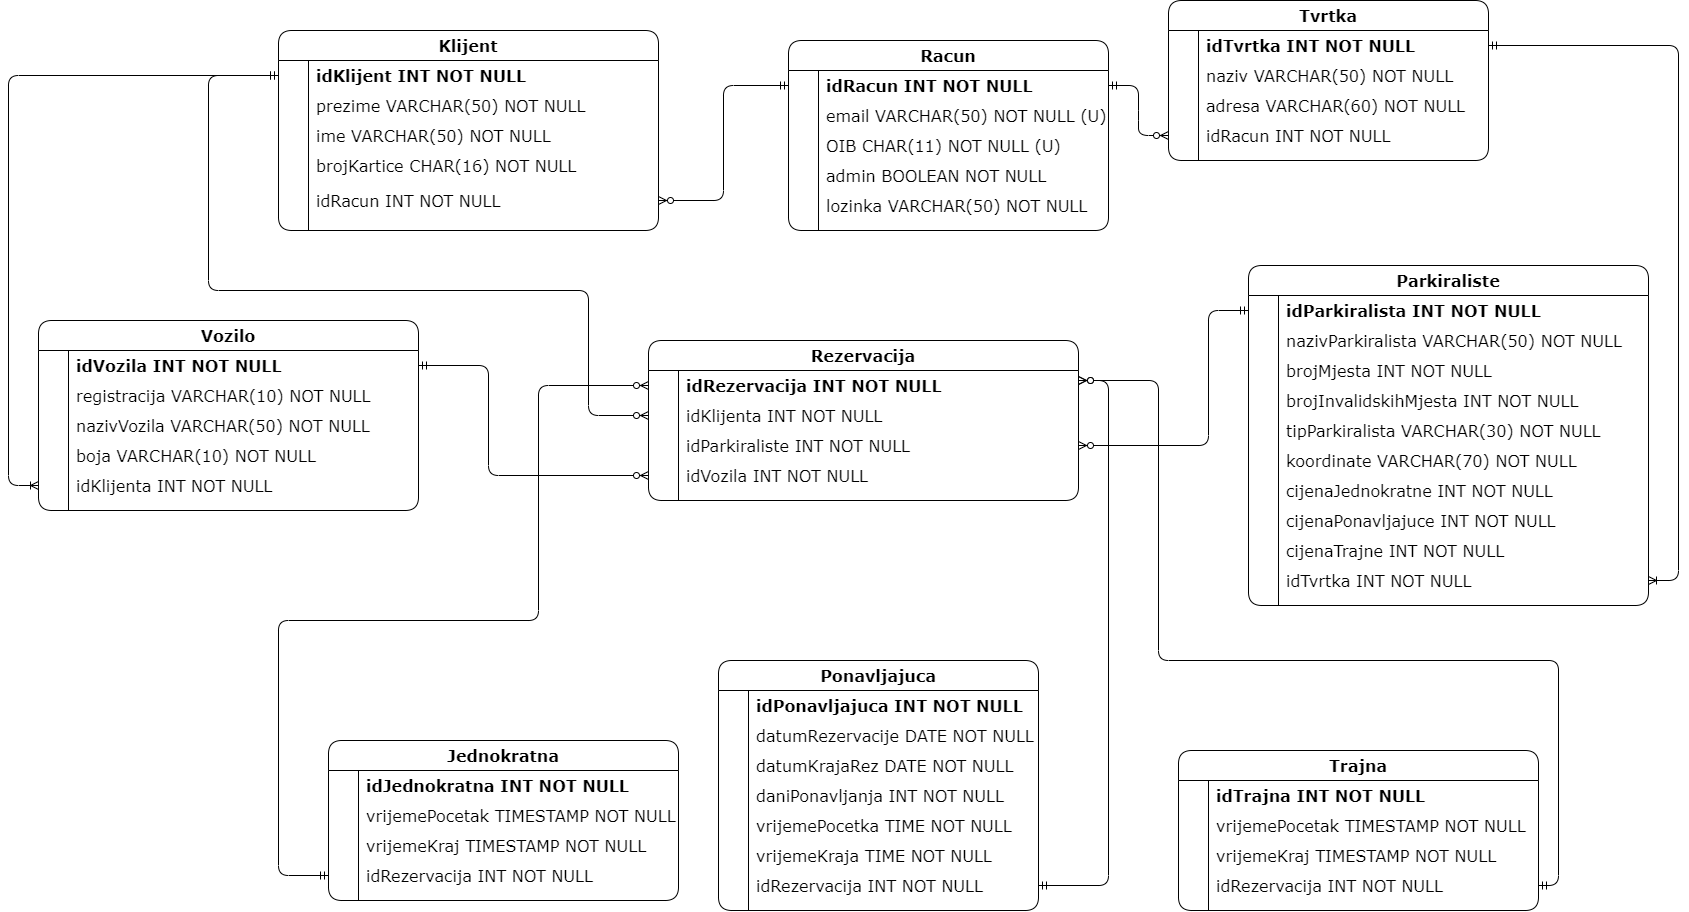
\includegraphics[width=1\linewidth]{dijagrami/ERModel.png} %veličina u odnosu na širinu linije
                	\caption{Prikaz funkcionalnosti vezanih za korisničke podatke}
                	\label{fig:promjene2} %label mora biti drugaciji za svaku sliku
                \end{figure}
			
			\eject
			
			
		\section{Dijagram razreda}
		
			\textit{Potrebno je priložiti dijagram razreda s pripadajućim opisom. Zbog preglednosti je moguće dijagram razlomiti na više njih, ali moraju biti grupirani prema sličnim razinama apstrakcije i srodnim funkcionalnostima.}\\
			
			\textbf{\textit{dio 1. revizije}}\\
			
			\textit{Prilikom prve predaje projekta, potrebno je priložiti potpuno razrađen dijagram razreda vezan uz \textbf{generičku funkcionalnost} sustava. Ostale funkcionalnosti trebaju biti idejno razrađene u dijagramu sa sljedećim komponentama: nazivi razreda, nazivi metoda i vrste pristupa metodama (npr. javni, zaštićeni), nazivi atributa razreda, veze i odnosi između razreda.}\\
			
			\textbf{\textit{dio 2. revizije}}\\			
			
			\textit{Prilikom druge predaje projekta dijagram razreda i opisi moraju odgovarati stvarnom stanju implementacije}
			
			
			
			\eject
		
		\section{Dijagram stanja}
			
			
			\textbf{\textit{dio 2. revizije}}\\
			
			\textit{Potrebno je priložiti dijagram stanja i opisati ga. Dovoljan je jedan dijagram stanja koji prikazuje \textbf{značajan dio funkcionalnosti} sustava. Na primjer, stanja korisničkog sučelja i tijek korištenja neke ključne funkcionalnosti jesu značajan dio sustava, a registracija i prijava nisu. }
			
			
			\eject 
		
		\section{Dijagram aktivnosti}
			
			\textbf{\textit{dio 2. revizije}}\\
			
			 \textit{Potrebno je priložiti dijagram aktivnosti s pripadajućim opisom. Dijagram aktivnosti treba prikazivati značajan dio sustava.}
			
			\eject
		\section{Dijagram komponenti}
		
			\textbf{\textit{dio 2. revizije}}\\
		
			 \textit{Potrebno je priložiti dijagram komponenti s pripadajućim opisom. Dijagram komponenti treba prikazivati strukturu cijele aplikacije.}
	\chapter{Implementacija i korisničko sučelje}

		
		\section{Korištene tehnologije i alati}
		
			Komunikacija u timu realizirana je korištenjem aplikacije \underline{WhatsApp} \footnote{\href{https://www.whatsapp.com/}{Whatsapp}} za manje i kraće dogovore, a za dulje i veće dogovore komunikacija je realizirana korištenjem aplikacije \underline{Microsoft Teams} \footnote{\href{https://www.microsoft.com/hr-hr/microsoft-365/microsoft-teams/group-chat-software}{Microsoft Teams}}. Za izradu UML dijagrama korišten je alat \underline{Astah UML} \footnote{\href{https://astah.net/products/astah-uml/}{Astah UML}}. Kao sustav za upravljanje izvornim kodom Git \footnote{\href{https://git-scm.com/}{Git}}. Udaljeni repozitorij projekta je dostupan na web platformi \underline{GitLab} \footnote{\href{https://www.gitlab.com}{Gitlab}}.

			Kao razvojno okruženje korišten je \underline{Microsoft Visual Studio Code} \footnote{\href{https://code.visualstudio.com/}{Microsoft Visual Studio Code}}. Microsoft Visual Studio Code trenutno je \underline{najpopularnije} \footnote{\href{https://pypl.github.io/IDE.html}{Deset najraširenijih razvojnih okruženja}} razvojno okruženje, iznimno je prilagodljiv raznim potrebama programera i potrebama samog programskog jezika.
			
			Aplikacija je izrađena u dva dijela. Backend dio je napisan koristeći radni okvir \underline{Express.js} \footnote{\href{https://expressjs.com/}{Express.js}} u programskom jeziku \underline{TypeScript} \footnote{\href{https://www.typescriptlang.org/}{TypeScript}}, a frontend dio je napisan koristeći biblioteku \underline{React.js} \footnote{\href{https://reactjs.org/}{React.js}} u programskom jeziku \underline{JavaScript} \footnote{\href{https://www.javascript.com/}{JavaScript}}.
			
			Express.js radni okvir je javno dostupan, besplatan te otvorenog izvora pružen od strane \underline{OpenJS Foundation-a} \footnote{\href{https://openjsf.org/}{OpenJS Foundation}}. Express.js je jednostavna i prilagodljiv \underline{Node.js}\footnote{\href{https://nodejs.org/en/}{Node.js}} radni okvir koja pruža izdržljiv skup značajki za web i mobilne aplikacije.
			
			React.js je JavaScript biblioteka za izradu interaktivnih sučelja unutar web aplikacija. Održavana je od strane Facebooka, a najčešće je korišten kao osnova u razvoju web aplikacija.
			
			Korištena baza podataka je \underline{PostgreSQL} \footnote{\href{https://www.postgresql.org/}{PostgreSQL}}. PostgreSQL je besplatna, objektno-relacijska baza podataka sa više od 30 godina aktivnog razvoja.
			
			Cijela aplikacija poslužena je na \underline{Heroku} \footnote{\href{https://www.heroku.com/home}{Heroku}}. Heroku je platforma koja omogućuje jednostavno i sigurno puštanje  u pogon i nadziranje aplikacija. Konkretno, koristimo dvije Heroku aplikacije, jednu za backend i jednu za frontend te u sklopu backend aplikacije koristimo i jednu instancu PostrgeSQL baze podataka.
			
			\eject 
		
	
		\section{Ispitivanje programskog rješenja}
			
			\textbf{\textit{dio 2. revizije}}\\
			
			 \textit{U ovom poglavlju je potrebno opisati provedbu ispitivanja implementiranih funkcionalnosti na razini komponenti i na razini cijelog sustava s prikazom odabranih ispitnih slučajeva. Studenti trebaju ispitati temeljnu funkcionalnost i rubne uvjete.}
	
			
			\subsection{Ispitivanje komponenti}
			\textit{Potrebno je provesti ispitivanje jedinica (engl. unit testing) nad razredima koji implementiraju temeljne funkcionalnosti. Razraditi \textbf{minimalno 6 ispitnih slučajeva} u kojima će se ispitati redovni slučajevi, rubni uvjeti te izazivanje pogreške (engl. exception throwing). Poželjno je stvoriti i ispitni slučaj koji koristi funkcionalnosti koje nisu implementirane. Potrebno je priložiti izvorni kôd svih ispitnih slučajeva te prikaz rezultata izvođenja ispita u razvojnom okruženju (prolaz/pad ispita). }
			
			
			
			\subsection{Ispitivanje sustava}
			
			 \textit{Potrebno je provesti i opisati ispitivanje sustava koristeći radni okvir Selenium\footnote{\url{https://www.seleniumhq.org/}}. Razraditi \textbf{minimalno 4 ispitna slučaja} u kojima će se ispitati redovni slučajevi, rubni uvjeti te poziv funkcionalnosti koja nije implementirana/izaziva pogrešku kako bi se vidjelo na koji način sustav reagira kada nešto nije u potpunosti ostvareno. Ispitni slučaj se treba sastojati od ulaza (npr. korisničko ime i lozinka), očekivanog izlaza ili rezultata, koraka ispitivanja i dobivenog izlaza ili rezultata.\\ }
			 
			 \textit{Izradu ispitnih slučajeva pomoću radnog okvira Selenium moguće je provesti pomoću jednog od sljedeća dva alata:}
			 \begin{itemize}
			 	\item \textit{dodatak za preglednik \textbf{Selenium IDE} - snimanje korisnikovih akcija radi automatskog ponavljanja ispita	}
			 	\item \textit{\textbf{Selenium WebDriver} - podrška za pisanje ispita u jezicima Java, C\#, PHP koristeći posebno programsko sučelje.}
			 \end{itemize}
		 	\textit{Detalji o korištenju alata Selenium bit će prikazani na posebnom predavanju tijekom semestra.}
			
			\eject 
		
		
		\section{Dijagram razmještaja}
			
			\textbf{\textit{dio 2. revizije}}
			
			 \textit{Potrebno je umetnuti \textbf{specifikacijski} dijagram razmještaja i opisati ga. Moguće je umjesto specifikacijskog dijagrama razmještaja umetnuti dijagram razmještaja instanci, pod uvjetom da taj dijagram bolje opisuje neki važniji dio sustava.}
			
			\eject 
		
		\section{Upute za puštanje u pogon}
		
			\textbf{\textit{dio 2. revizije}}\\
		
			 \textit{U ovom poglavlju potrebno je dati upute za puštanje u pogon (engl. deployment) ostvarene aplikacije. Na primjer, za web aplikacije, opisati postupak kojim se od izvornog kôda dolazi do potpuno postavljene baze podataka i poslužitelja koji odgovara na upite korisnika. Za mobilnu aplikaciju, postupak kojim se aplikacija izgradi, te postavi na neku od trgovina. Za stolnu (engl. desktop) aplikaciju, postupak kojim se aplikacija instalira na računalo. Ukoliko mobilne i stolne aplikacije komuniciraju s poslužiteljem i/ili bazom podataka, opisati i postupak njihovog postavljanja. Pri izradi uputa preporučuje se \textbf{naglasiti korake instalacije uporabom natuknica} te koristiti što je više moguće \textbf{slike ekrana} (engl. screenshots) kako bi upute bile jasne i jednostavne za slijediti.}
			
			
			 \textit{Dovršenu aplikaciju potrebno je pokrenuti na javno dostupnom poslužitelju. Studentima se preporuča korištenje neke od sljedećih besplatnih usluga: \href{https://aws.amazon.com/}{Amazon AWS}, \href{https://azure.microsoft.com/en-us/}{Microsoft Azure} ili \href{https://www.heroku.com/}{Heroku}. Mobilne aplikacije trebaju biti objavljene na F-Droid, Google Play ili Amazon App trgovini.}
			
			
			\eject 
	\chapter{Zaključak i budući rad}
		
		Naš je zadatak bio napraviti web aplikaciju koja će korisnicima omogućiti pretraživanje i rezervaciju slobodnih parkirališnih mjesta u gradu Zagrebu svih tvrtki koje odluče nuditi parkiralište preko naše aplikacije. 
		
		Rad na aplikaciji podijelili smo u dvije faze: planiranje i izrada dokumentacije i generičkih funkcionalnosti aplikacije te implementacija projekta, ispitivanje i dovršetak dokumentacije.
		
		Prvu fazu započeli smo okupljanjem razvojnog tima. Nakon što smo dobili projektni zadatak, počeli smo s dokumentiranjem i dogovaranjem kako će naša aplikacija izgledati. Tu smo naišli i na prve izazove. Nitko od nas nije radio sličan projekt i nije znao što očekivati niti kako započeti rad na takvom projektu. Mislili smo da trebamo što prije početi programirati, ali čim smo započeli shvatili smo kako prvo trebamo dobro definirati svojstva naše aplikacije, sve zahtjeve i moguće scenarije pa smo to i napravili. Izrađena dokumentacija (obrasci uporabe, dijagram baze podataka itd.) pomogla nam je da se bolje upoznamo sa zadatkom, a kasnije nudila jasne smjernice kako bi naša aplikacija trebala izgledati.
		
		Podijelili smo se u tri grupe koje su radile na određenim dijelovima aplikacije: frontend, backend i baze podataka. Grupa zadužena za bazu podataka se nakon izrade baze pridružila \textit{backendu} i \textit{frontendu}. Prvu smo fazu završili implementacijom registracije i prijave za korisnike.
		
		Druga faza većinom se sastojala od implementacije aplikacije. Jasno definirani zahtjevi napisani u dokumentaciji ubrzali su rad na aplikaciji. Svatko je znao što treba raditi i kako bi to trebalo izgledati na kraju. Na kraju druge faze dovršili smo ispitivanje aplikacije i preostalu dokumentaciju koja će poslužiti za buduće inačice sustava.
		
		Radeći na ovom projektu morali smo riješiti mnoge izazove. Koristili smo potpuno nove tehnologije koje smo prvo morali naučiti da bi ih dobro upotrijebili. Implementacija karte, postavljanje aplikacije na javno dostupnom poslužitelju, komunikacija baze podataka, \textit{backend} i \textit{frontend} dijela samo su neki od izazova koje smo uspješno savladali. Naučili smo raditi u grupi, rješavati konflikte, koristiti nove tehnologije i ne bojati se probati nešto novo. 
		
		Neki izazovi su bili tehnički prezahtjevni za nas da ih riješimo u okviru ovog zadatka. Javni web poslužitelj kojeg smo koristili ne omogućuje nam da dohvaćamo trenutnu lokaciju korisnika i spremamo kolačiće na njegovu domenu. Spremanje kolačića smo riješili kupnjom vlastite domene, dok dohvaćanje trenutne lokacije sigurno ostaje kao daljnja mogućnost poboljšanja aplikacije. Uz to, poboljšanje ove aplikacije može se ostvariti izgradnjom mobilne aplikacije što je jedan od budućih proširenja sustava.
		
		Ovaj projektni zadatak bio je vrijedno iskustvo svim članovima grupe. Iskusili smo kako je biti dio tima, raditi stvari u zadanom roku. Naučili smo koliko dobra organizacija i priprema pomažu i ubrzavaju rad na projektu, ali i koliko još imamo za učiti i da će uvijek biti mjesta za napredak.
		
		\eject 
	\chapter*{Popis literature}
		\addcontentsline{toc}{chapter}{Popis literature}
	 	
 		\textbf{\textit{Kontinuirano osvježavanje}}
	
		\textit{Popisati sve reference i literaturu koja je pomogla pri ostvarivanju projekta.}
		
		
		\begin{enumerate}
			
			
			\item  Programsko inženjerstvo, FER ZEMRIS, \url{http://www.fer.hr/predmet/proinz}
			
			\item  I. Sommerville, "Software engineering", 8th ed, Addison Wesley, 2007.
			
			\item  T.C.Lethbridge, R.Langaniere, "Object-Oriented Software Engineering", 2nd ed. McGraw-Hill, 2005.
			
			\item  I. Marsic, Software engineering book``, Department of Electrical and Computer Engineering, Rutgers University, \url{http://www.ece.rutgers.edu/~marsic/books/SE}
			
			\item  The Unified Modeling Language, \url{https://www.uml-diagrams.org/}
			
			\item  Astah Community, \url{http://astah.net/editions/uml-new}
		\end{enumerate}
		
		 
	
	
	\begingroup
	\renewcommand*\listfigurename{Indeks slika i dijagrama}
	%\renewcommand*\listtablename{Indeks tablica}
	%\let\clearpage\relax
	\listoffigures
	%\vspace{10mm}
	%\listoftables
	\endgroup
	\addcontentsline{toc}{chapter}{Indeks slika i dijagrama}
	
	
	
	\eject 
	
	\chapter*{Dodatak: Prikaz aktivnosti grupe}
		\addcontentsline{toc}{chapter}{Dodatak: Prikaz aktivnosti grupe}
		
		\section*{Dnevnik sastajanja}
		
			\begin{packed_enum}
			\item  sastanak
			
			\item[] \begin{packed_item}
				\item Datum: 7.listopada.2020
				\item Prisustvovali: (Svi): M.Ćubela, K.Djaković, L.Matković, L.Strejček, A, Krišto, K.Petković, M.Bakić
				\item Teme sastanka: Inicijalni sastanak
				\begin{packed_item}
					\item Detalji o tehnologijama
					\item Git
					\item Latex
					\item Podjela tima na 3 pod tima
					\item Teme za sljedeći sastanak
				\end{packed_item}
			\end{packed_item}
			
			\item  sastanak
			\item[] \begin{packed_item}
				\item Datum: 9.listopada.2020
				\item Prisustvovali: Svi
				\item Teme sastanka: Odabir tehnologija za projekt
				\begin{packed_item}
					\item Odabir tehnologije
					\item AWS
					\item ORM
					\item JS
					\item Teme za sljedeći sastanak
				\end{packed_item}
			\end{packed_item}
			
				
			\item  sastanak
			\item[] \begin{packed_item}
				\item Datum: 10.listopada.2020
				\item Prisustvovali:  M.Ćubela, K. Djaković, K.Petković
				\item Teme sastanka: Inicijalizacija backenda
				\begin{packed_item}
					\item Dogovor o okvirnoj strukturi backenda
					\item Raspodjela poslova
					\item Pitanja za asistenticu
					\item Teme za sljedeći backend sastanak
				\end{packed_item}
			\end{packed_item}
			
			
			
			
			\item  sastanak
			\item[] \begin{packed_item}
				\item Datum: 10.listopada.2020
				\item Prisustvovali: K.Djaković, M.Bakić, M.Ćubela
				\item Teme sastanka: Proučavanje AWS-a
				\begin{packed_item}
					\item Izrada timskog računa (Gmail, AWS)
					\item Istrživanje mogućnosti "deploy"-a
					\item PostreSQL - AWS
				\end{packed_item}
			\end{packed_item}
			
			
			\item  sastanak
			\item[] \begin{packed_item}
				\item Datum: 12.listopada.2020
				\item Prisustvovali:  K.Djaković, M.Bakić
				\item Teme sastanka: Odabir tehnologija za projekt
				\begin{packed_item}
					\item Uspostava servera(AWS)
				\end{packed_item}
			\end{packed_item}
			
			\item  sastanak
			\item[] \begin{packed_item}
				\item Datum: 12.listopada.2020
				\item Prisustvovali:  M.Ćubela, K.Petković
				\item Teme sastanka: Podjela poslova na backendu
				\begin{packed_item}
					\item Pregled zadataka za backend
					\item Raspodjela poslova
					\item Pitanja za asistenticu
					\item Teme za sljedeći backend sastanak
				\end{packed_item}
			\end{packed_item}
			
			
			
			\item  sastanak
			\item[] \begin{packed_item}
				\item Datum: 14.listopada.2020
				\item Prisustvovali: Svi
				\item Teme sastanka: Okvirno definiranje zahtjeva
				\begin{packed_item}
					\item Funkcionalni zahtjevi
					\item Nedefinirane radnje
					\item Pitanja za asistenticu
					\item Teme za sljedeći sastanak
				\end{packed_item}
			\end{packed_item}
			
				
			\item  sastanak
			\item[] \begin{packed_item}
				\item Datum: 16.listopada.2020
				\item Prisustvovali: Svi
				\item Teme sastanka: Pregled dosadašnjeg napretka
				\begin{packed_item}
					\item Pregled primjera projektne dokumentacije
					\item Povezivanje entiteta u bazi
					\item Pitanja za asistenticu
					\item Teme za sljedeći sastanak
				\end{packed_item}
			\end{packed_item}
			
			
			
			\item  sastanak
			\item[] \begin{packed_item}
				\item Datum: 21.listopada.2020
				\item Prisustvovali: Svi
				\item Teme sastanka: Pregled dosadašnjeg napretka
				\begin{packed_item}
				    \item Pregled napretka
					\item Podjela zadataka u vezi dokumentacije
					\item Teme za sljedeći sastanak
				\end{packed_item}
			\end{packed_item}
			
			
			\item  sastanak
			\item[] \begin{packed_item}
				\item Datum: 28.listopada.2020
				\item Prisustvovali: K.Djaković, L.Matković, M.Bakić, L.Strejček
				\item Teme sastanka: Podizanje baze, Heroku
				\begin{packed_item}
				    \item Prebacivanje s AWS na Heroku
					\item Izrada računa
					\item Podizanje servera na Heroku
				\end{packed_item}
			\end{packed_item}
			
			\item  sastanak
			\item[] \begin{packed_item}
				\item Datum: 27.listopada.2020
				\item Prisustvovali: L.Strejček, A.Krišto
				\item Teme sastanka: Izrada ER modela
				\begin{packed_item}
				    \item Definiranje i izrada ER modela
					\item Pregledavanje baze
					\item Podjela zadataka
					\item Pitanja za asistenticu
					\item Teme za sljedeći sastanak
				\end{packed_item}
			\end{packed_item}
			
			\item  sastanak
			\item[] \begin{packed_item}
				\item Datum: 30.listopada.2020
				\item Prisustvovali: Svi
				\item Teme sastanka: Pregled dosadašnjeg napretka
				\begin{packed_item}
				    \item Dogovor o nesuglasnostima
					\item Entitet "administrator"
					\item Odluka o korištenju ORM-a
					\item UML dijagrami
					\item UC - ovi
					\item Podjela zadataka
					\item Pitanja za asistenticu
				\end{packed_item}
			\end{packed_item}
			
			
			\item  sastanak
			\item[] \begin{packed_item}
				\item Datum: 3.studeni.2020
				\item Prisustvovali: L.Strejček, A.Krišto
				\item Teme sastanka: Izrada ER modela
				\begin{packed_item}
				    \item Definiranje i izrada ER modela
					\item Pregledavanje baze
					\item Podjela zadataka
					\item Pitanja za asistenticu
					\item Teme za sljedeći sastanak
				\end{packed_item}
			\end{packed_item}
			
			\item  sastanak
			\item[] \begin{packed_item}
				\item Datum: 4.studeni.2020
				\item Prisustvovali: Svi
				\item Teme sastanka: Pregled dosadašnjeg napretka
				\begin{packed_item}
				    \item Proučavanje ORM-a
					\item Podjela zadataka
					\item Pitanja za asistenticu
				\end{packed_item}
			\end{packed_item}
			
				\item  sastanak
			\item[] \begin{packed_item}
				\item Datum: 5.studeni.2020
				\item Prisustvovali: L.Strejček, A.Krišto
				\item Teme sastanka: Dokumentacija baze
				\begin{packed_item}
				    \item Pregled strukture dokumentacije
					\item Raspodjela poslova
					\item Pitanja za asistenticu
					\item Teme za sljedeći sastanak
				\end{packed_item}
			\end{packed_item}
			
			\item  sastanak
			\item[] \begin{packed_item}
				\item Datum: 9.studeni.2020
				\item Prisustvovali: Svi
				\item Teme sastanka: Pregled dosadašnjeg napretka
				\begin{packed_item}
				    \item Pregled izvršenih zadataka
					\item Podjela zadataka
					\item Pitanja za asistenticu
					\item Teme za sljedeći sastanak
				\end{packed_item}
			\end{packed_item}
			
			\item  sastanak
			\item[] \begin{packed_item}
				\item Datum: 9.studeni.2020
				\item Prisustvovali: Svi + Nikolina Frid
				\item Teme sastanka: Prezentacija trenutnog stanja
				\begin{packed_item}
				    \item Prikaz stanja aplikacije
					\item Prikaz stanja dokumentacije
					\item Dogovor o koracima napretka
					\item Pitanja za asistenticu
				\end{packed_item}
			\end{packed_item}
			
			\item  sastanak
			\item[] \begin{packed_item}
				\item Datum: 12.studeni.2020
				\item Prisustvovali: Svi
				\item Teme sastanka: Pregled dokumentacije
				\begin{packed_item}
				    \item Provjera pogrešaka u dokumentaciji
					\item Pogreška u korištenoj tehnologiji za backend
					\item Dogovor o prebacivanju cijelog backenda u TypeScript
					\item Ispravljanje dokumentacije
					\item Podjela zadataka
					\item Pitanja za asistenticu
				\end{packed_item}
			\end{packed_item}
			
			\item  sastanak
			\item[] \begin{packed_item}
				\item Datum: 13.studeni.2020
				\item Prisustvovali: K.Djaković, M.Ćubela, K.Petković
				\item Teme sastanka: Restrukturiranje cijelokupnog backenda u OO paradigmu
				\begin{packed_item}
                    \item Dogovor o načinu prebacivanja u TypeScript
                    \item Raspodjela poslova prebacivanja
                    \item Pitanja za asistenticu
                    \item Dogovor za sljedeći sastanak
				\end{packed_item}
			\end{packed_item}
			
			\item  sastanak
			\item[] \begin{packed_item}
				\item Datum: 14.studeni.2020
				\item Prisustvovali: K.Djaković, M.Ćubela, K.Petković
				\item Teme sastanka: Pregled napretka restrukturiranja backenda
				\begin{packed_item}
                    \item Pregled napretka
                    \item Ispravak pogrešaka
                    \item Dogovor o načinu nastavljanja rekonstrukcije
                    \item Podjela poslova
				\end{packed_item}
			\end{packed_item}
			
				\item  sastanak
			\item[] \begin{packed_item}
				\item Datum: 22.studeni.2020
				\item Prisustvovali: Svi
				\item Teme sastanka: Pregled dosadašnjeg napretka
				\begin{packed_item}
				    \item Pregled izvršenih zadataka
					\item Podjela zadataka
					\item Pitanja za asistenticu
					\item Teme za sljedeći sastanak
				\end{packed_item}
			\end{packed_item}
			
				\item  sastanak
			\item[] \begin{packed_item}
				\item Datum: 27.studeni.2020
				\item Prisustvovali: Svi
				\item Teme sastanka: Pregled dosadašnjeg napretka
				\begin{packed_item}
				    \item Pregled izvršenih zadataka
					\item Podjela zadataka
					\item Pitanja za asistenticu
					\item Teme za sljedeći sastanak
				\end{packed_item}
			\end{packed_item}
			
			\item  sastanak
			\item[] \begin{packed_item}
				\item Datum: 3.prosinca.2020
				\item Prisustvovali: Svi + dr. sc. Nikolina Frid
				\item Teme sastanka: Kolokviranje prvog dijela projekta
				\begin{packed_item}
                    \item Prikaz aplikacije i dokumentacije
                    \item Ispitivanje pojedinačnih članova tipa
                    \item Isticanje pogrešaka
                    \item Dogovor za sljedeće napretke
				\end{packed_item}
			\end{packed_item}
			
				\item  sastanak
			\item[] \begin{packed_item}
				\item Datum: 7.prosinca.2020
				\item Prisustvovali: Svi
				\item Teme sastanka: Pregled dosadašnjeg napretka
				\begin{packed_item}
				    \item Pregled izvršenih zadataka
					\item Podjela zadataka
					\item Pitanja za asistenticu
					\item Teme za sljedeći sastanak
				\end{packed_item}
			\end{packed_item}
			
				\item  sastanak
			\item[] \begin{packed_item}
				\item Datum: 15.prosinca.2020
				\item Prisustvovali: Svi
				\item Teme sastanka: Pregled dosadašnjeg napretka
				\begin{packed_item}
				    \item Pregled izvršenih zadataka
					\item Podjela zadataka
					\item Pitanja za asistenticu
					\item Teme za sljedeći sastanak
				\end{packed_item}
			\end{packed_item}
			
				\item  sastanak
			\item[] \begin{packed_item}
				\item Datum: 22.prosinca.2020
				\item Prisustvovali: Svi
				\item Teme sastanka: Pregled dosadašnjeg napretka
				\begin{packed_item}
				    \item Pregled izvršenih zadataka
					\item Podjela zadataka
					\item Pitanja za asistenticu
					\item Teme za sljedeći sastanak
				\end{packed_item}
			\end{packed_item}
			
			
				\item  sastanak
			\item[] \begin{packed_item}
				\item Datum: 3.siječnja.2021
				\item Prisustvovali: Svi
				\item Teme sastanka: Pregled dosadašnjeg napretka
				\begin{packed_item}
				    \item Pregled izvršenih zadataka
					\item Podjela zadataka
					\item Pitanja za asistenticu
					\item Teme za sljedeći sastanak
				\end{packed_item}
			\end{packed_item}
			
				\item  sastanak
			\item[] \begin{packed_item}
				\item Datum: 7.siječnja.2021
				\item Prisustvovali: Svi
				\item Teme sastanka: Sastanak prije demonstracije alpha inačice
				\begin{packed_item}
                    \item Pregled aplikacije
                    \item Pregled dokumentacije
                    \item Ispravljanje detalja
                    \item Pitanja za asistenticu
				\end{packed_item}
			\end{packed_item}
			
			\item  sastanak
			\item[] \begin{packed_item}
				\item Datum: 8.siječnja.2021
				\item Prisustvovali: Svi + dr. sc. Nikolina Frid
				\item Teme sastanka: Demonstracija alpha inačice
				\begin{packed_item}
                    \item Demonstracija aplikacije
                    \item Prikaz dokumentacije
                    \item Sljedeći koraci
				\end{packed_item}
			\end{packed_item}
			
			\item  sastanak
			\item[] \begin{packed_item}
				\item Datum: 12.siječnja.2021
				\item Prisustvovali: Svi
				\item Teme sastanka: Pregled dosadašnjeg napretka
				\begin{packed_item}
				    \item Pregled izvršenih zadataka
					\item Podjela zadataka
					\item Teme za sljedeći sastanak
				\end{packed_item}
			\end{packed_item}
			
			\item  sastanak
			\item[] \begin{packed_item}
				\item Datum: 14.siječnja.2021
				\item Prisustvovali: Svi
				\item Teme sastanka: Pregled dosadašnjeg napretka
				\begin{packed_item}
				    \item Pregled izvršenih zadataka
				    \item Pregled dokumentacije
					\item Podjela zadataka
					\item Teme za sljedeći sastanak
				\end{packed_item}
			\end{packed_item}
			
				\item  sastanak
			\item[] \begin{packed_item}
				\item Datum: 15.siječnja.2021
				\item Prisustvovali: Svi
				\item Teme sastanka: Pregled dokumentacije
				\begin{packed_item}
				    \item Pregled dokumentacije
					\item Podjela zadataka nadopune i ispravaka
					\item Termin za sljedeći sastanak
				\end{packed_item}
			\end{packed_item}
			
				\item  sastanak
			\item[] \begin{packed_item}
				\item Datum: 18.siječnja.2021
				\item Prisustvovali: Svi
				\item Teme sastanka: Sastanak prije kolokviranja
				\begin{packed_item}
				    \item Pregled cjelokupnog projekta
					\item Završni ispravci
				\end{packed_item}
			\end{packed_item}
			
			
			\item  sastanak
			\item[] \begin{packed_item}
				\item Datum: 20.siječnja.2021
				\item Prisustvovali: Svi + dr. sc. Nikolina Frid
				\item Teme sastanka: Kolokviranje projekta
				\begin{packed_item}
                    \item Demonstracija završne aplikacije
                    \item Završna dokumentacija
                    \item Pojedinačno ispitivanje članova tima
				\end{packed_item}
			\end{packed_item}
			
			
			
			%
			
		\end{packed_enum}
		\eject
		\section*{Tablica aktivnosti}

			\begin{longtabu} to \textwidth {|X[7, l]|X[1, c]|X[1, c]|X[1, c]|X[1, c]|X[1, c]|X[1, c]|X[1, c]|}
								
				\cline{2-8} \multicolumn{1}{c|}{\textbf{}} &     \multicolumn{1}{c|}{\rotatebox{90}{\textbf{Marin Ćubela }}} & \multicolumn{1}{c|}{\rotatebox{90}{\textbf{Marko Bakić }}} &	\multicolumn{1}{c|}{\rotatebox{90}{\textbf{Kristian Djaković }}} &	\multicolumn{1}{c|}{\rotatebox{90}{\textbf{Andrea Krišto }}} &
				\multicolumn{1}{c|}{\rotatebox{90}{\textbf{Lea Matković }}} &
				\multicolumn{1}{c|}{\rotatebox{90}{\textbf{Kristina Petković }}} &	\multicolumn{1}{c|}{\rotatebox{90}{\textbf{Lucija Strejček }}} \\ \hline 
				\endfirsthead
				
			
				\cline{2-8} \multicolumn{1}{c|}{\textbf{}} &     \multicolumn{1}{c|}{\rotatebox{90}{\textbf{Marin Ćubela }}} & \multicolumn{1}{c|}{\rotatebox{90}{\textbf{Marko Bakić }}} &	\multicolumn{1}{c|}{\rotatebox{90}{\textbf{Kristian Djaković }}} &	\multicolumn{1}{c|}{\rotatebox{90}{\textbf{Andrea Krišto }}} &
				\multicolumn{1}{c|}{\rotatebox{90}{\textbf{Lea Matković }}} &
				\multicolumn{1}{c|}{\rotatebox{90}{\textbf{Kristina Petković }}} &	\multicolumn{1}{c|}{\rotatebox{90}{\textbf{Lucija Strejček }}} \\ \hline  
				\endhead
				
				
				\endfoot
							
				 
				\endlastfoot
				
				Upravljanje projektom 		&8  &  &  &  &  &  & \\ \hline
				Opis projektnog zadatka 	&  &  &  &  &4  &  &4 \\ \hline
				
				Funkcionalni zahtjevi       &1  &3  &3  &1  &1  &3  &1  \\ \hline
				Opis pojedinih obrazaca 	&2  &6  &6  &6  &6  &6  &6  \\ \hline
				Dijagram obrazaca 			&4  &  &  &4  &  &  &  \\ \hline
				Sekvencijski dijagrami 		&  &  &5  &  &4  &  &4  \\ \hline
				Opis ostalih zahtjeva 		&  &  &  &  &  &4  &  \\ \hline

				Arhitektura i dizajn sustava	 &  &2  &  &  &  &4  &  \\ \hline
				Baza podataka				&1  &1  &  &4  &  &  &4   \\ \hline
				Dijagram razreda 			&5  &10  &  &10  &  &  &   \\ \hline
				Dijagram stanja				&  &  &3  &  &4  &  &  \\ \hline
				Dijagram aktivnosti 		&  &  &  &  &3  &  &3  \\ \hline
				Dijagram komponenti			&  &  &  &  &3  &  &3  \\ \hline
				Korištene tehnologije i alati 		&  &  &4  &  &  &  &  \\ \hline
				Ispitivanje programskog rješenja 	&2  &  &  &  &  &5  &  \\ \hline
				Dijagram razmještaja			&  &  &  &  &  &3  &  \\ \hline
				Upute za puštanje u pogon 		&  &  &4  &  &  &  &  \\ \hline 
				Dnevnik sastajanja 			&  &3  &  &  &  &  &  \\ \hline
				Zaključak i budući rad 		&2  &  &  &  &  &  &  \\  \hline
				Popis literature 			&  &  &  &  &  &  &  \\  \hline
				
				\textbf{Dodatne funkcionalnosti} 	&  &  &  &  &  &  & \\ \hline
				\textit{izrada baze podataka} 	&  &  &  &20  &  &  &20 \\ \hline 
				\textit{izrada frontend-a} 		&  &130  &60  &  &140  &  &120  \\ \hline 
				\textit{izrada backend-a} 		&140  &  &60  &120  &  &140  &  \\  \hline
				\textit{deploy aplikacije} 		&  &10  &20  &  &  &  &  \\ \hline
				
				
			\end{longtabu}
					
					
		\eject
		\section*{Dijagrami pregleda promjena}
		
		\textbf{\textit{dio 2. revizije}}\\
		
		\textit{Prenijeti dijagram pregleda promjena nad datotekama projekta. Potrebno je na kraju projekta generirane grafove s gitlaba prenijeti u ovo poglavlje dokumentacije. Dijagrami za vlastiti projekt se mogu preuzeti s gitlab.com stranice, u izborniku Repository, pritiskom na stavku Contributors.}
		
	
	
	
\end{document} %naredbe i tekst nakon ove naredbe ne ulaze u izgrađen dokument 